\section{Type 4}
\begin{figure}[htbp]
\centering
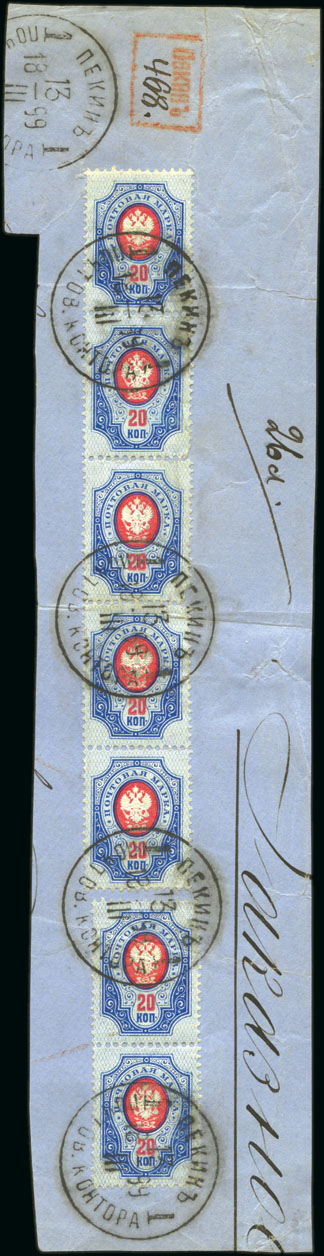
\includegraphics[width=.60\textwidth]{../russian-post-offices-in-china/10028.jpg}
\caption{
10028	PEKING: Large fragment with seven 20k tied by Peking 13.3.99 cds (T\&S type 4) 
with primitive boxed registration cachet in red adjacent with "PEKING" 
and ms number, this cachet preceded the registration labels, and is one 
of three examples known.
\euro 400.00 
}  
\end{figure}

\section{Type 4}
\begin{figure}[htbp]
\centering
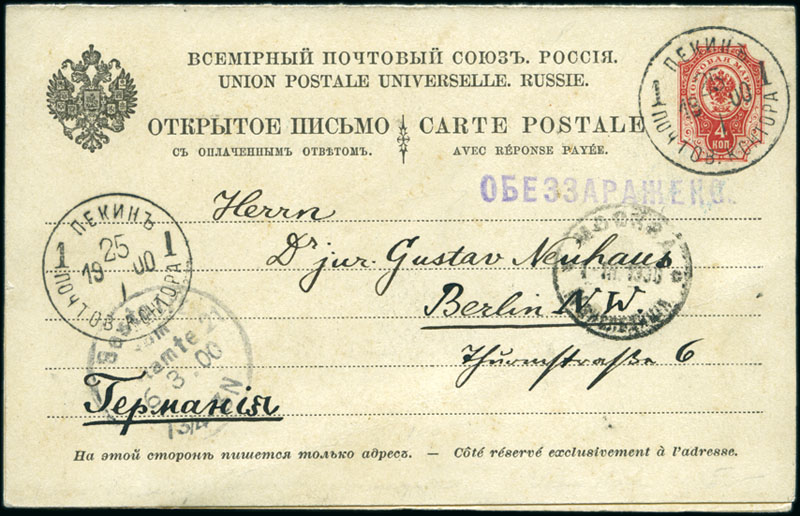
\includegraphics[width=.95\textwidth]{../russian-post-offices-in-china/10029.jpg}
\caption{
10029		ZoomPEKING: 1900 4k (+4k) Reply-paid postcard (reply portion unused) to 
Germany, cancelled by Peking 25.1.00 cds (T\&S type 4), with violet disinfection 
mark OBEZZARAZHEHO of Troitskosavsk adjacent with Moscow and arrival cds, very fine.
Note: Disinfection of mail from China was carried out at Russian frontier 
posts intermittently between 1895 and 1900 in response to cholera epidemics
\euro 500.00 
}  
\end{figure}

\begin{figure}[htbp]
\centering
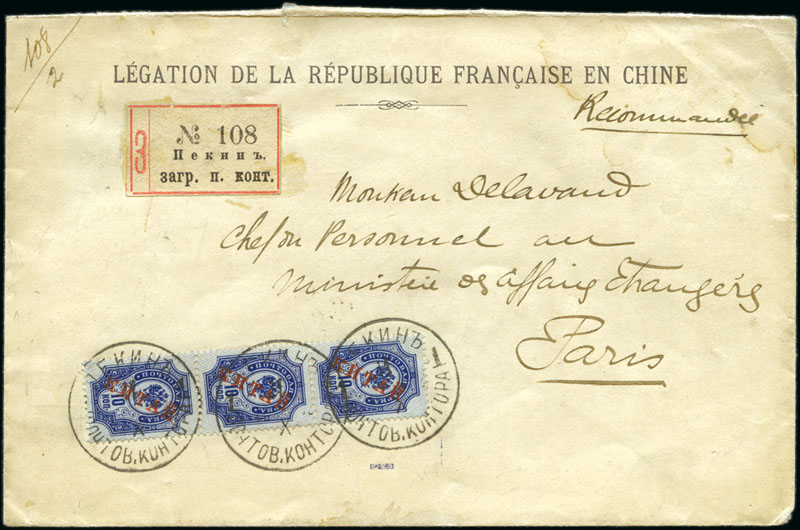
\includegraphics[width=.95\textwidth]{../russian-post-offices-in-china/10030.jpg}
\caption{
10030 PEKING: 1902 Printed envelope from the French Legation in China registered 
to France, with vertical strip of three "KITAI" 10k tied by Peking 11.10.02 
(T\&S type 6) with "Peking / Post Office Abroad" registered label in Cyrillic, 
Paris bs

\euro 700.00 
}  
\end{figure}

\begin{figure}[htbp]
\centering
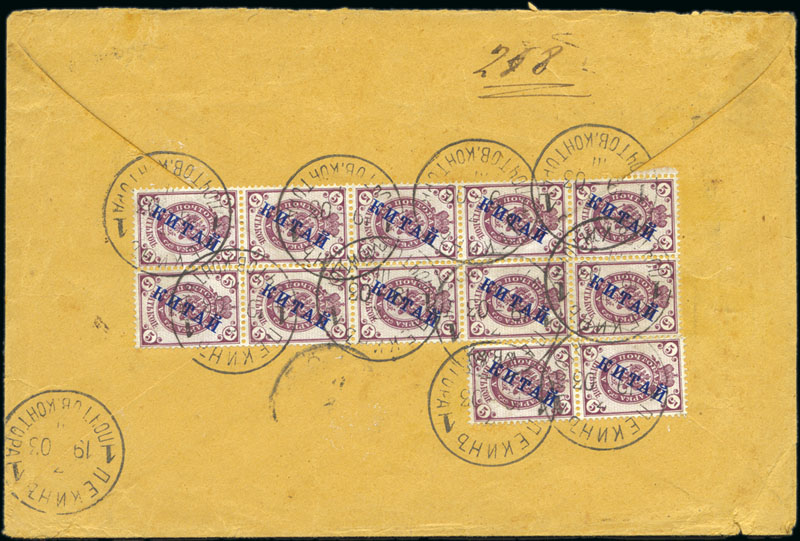
\includegraphics[width=.95\textwidth]{../russian-post-offices-in-china/10031.jpg}
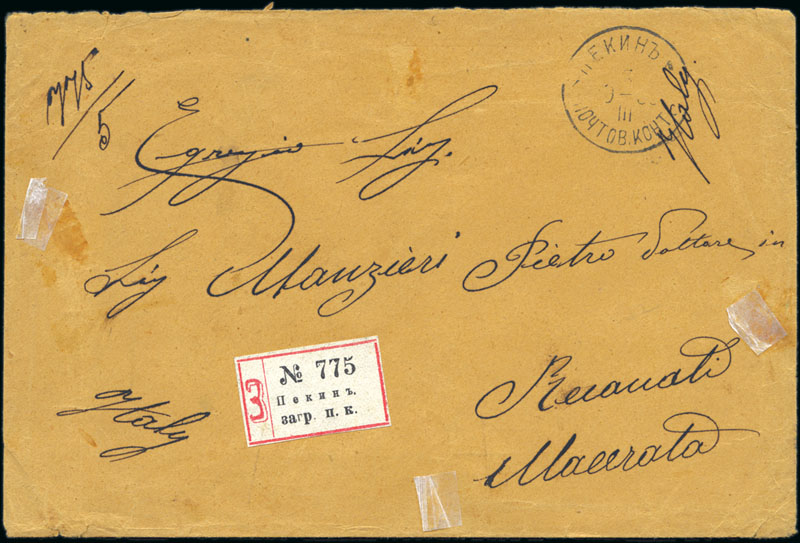
\includegraphics[width=.95\textwidth]{../russian-post-offices-in-china/10031-1.jpg}
\caption{
10031 PEKING: 1903 Cover to Italy franked on the reverse with "KITAI" 5k
in irregular block of twelve, paying five times the 10k rate plus reg'n fee,
tied by Peking 3.3.03 cds (T\&S type 6), with "Peking / Post Office Abroad"
registered label on the obverse, a rare large multiple on cover
\euro 400.00
}  
\end{figure}





                          